\section{Konzeption und Umsetzung}
\label{sec:4}

Für die Implementierung und Evaluierung der Performance der beiden beschriebenen Methoden wurde ein System mit den folgenden Spezifikationen verwendet:

\begin{table}[h]
	\renewcommand*{\arraystretch}{2}
	\setlength{\tabcolsep}{1.5cm}
	\begin{tabular}{lll}
		\hspace{-1.5cm}Betriebssystem & Win10 64-Bit                             \\ \hline
		\hspace{-1.5cm}Prozessor      & Intel(R) Core(TM) i5-9600K CPU @ 3.70GHz \\ \hline
		\hspace{-1.5cm}RAM            & 16GB                                     \\ \hline
		\hspace{-1.5cm}Grafikkarte    & NVIDIA GeForce RTX 2080 Ti               \\ \hline
		\hspace{-1.5cm}Speicher       & Samsung SSD 970 EVO Plus 500GB           \\ \hline
	\end{tabular}
	\caption{Spezifikationen des Computers, der im Rahmen dieser Arbeit verwendet wurde.}
\end{table}

\subsection{Idee}
\label{sec:4.1}

Da die Ergebnisse dieser Arbeit relevant für das KoViTReK Forschungsprojekt\footnote{\url{https://www.th-koeln.de/anlagen-energie-und-maschinensysteme/kovitrek\_87259.php}}
sein könnten und dieses in der Laufzeit- und Entwicklungsumgebung Unity\footnote{\url{https://unity.com}}
implementiert werden soll, werden auch die Partikelsysteme in der selben Umgebung entworfen.
Aufgrund der verschiedenen visuellen Eigenschaften und des Verhaltens von Feuer und Rauch werden jeweils eigene Systeme konzipiert.

Ein wichtiger Faktor bei der Darstellung von Rauch ist die Beleuchtung. Eigenschaften wie Streuungen und Reflexionen innerhalb des Mediums zu simulieren ist
aufwändig zu berechnen und unter Berücksichtigung aller Faktoren eher weniger für die Echtzeitberechung in VR-Systemen gedacht, welche deutlich höhere Anforderungen an die Performance der Anwendung
haben. Der erste Ansatz basiert auf einer Idee von Mederic Chasse, Technical Art Director  bei Highwire Games.
Dieser beschreibt im Forum \textit{realtimevfx.com} einen Workflow, mit dem aufwändige Berechnungen solcher Simulationen in einer VFX Software erstellt, durchsimuliert und in Texturen gebacken
werden können.
Die Animation wird in einem Texture Sheet gespeichert und kann somit eine realistische Darstellung bieten, während der Einsatz in einer Game Engine effizient bleibt \parencite{Chasse2018}.
Da der Fokus dieser Arbeit nicht auf der Fluidsimulation liegt und das Setup der Simulation mithilfe von Anleitungen
und Tipps artistischer Natur aus Internetforen erzeugt wird, wird an dieser Stelle nicht weiter darauf eingegangen, wie die VFX-Software den Rauch berechnet und erzeugt.
Stattdessen wird in \textbf{\autoref{sec:4.2.1}} der Workflow beschrieben und auf einige Parameter der Simulation eingegangen.

Für die Darstellung durch Ray Marching werden richtige Volumendaten, bzw. 3D-Texturen benötigt. Diese werden innerhalb von Unity
per Shader prozedural erzeugt.

<<<<TODO>>>>


\subsection{Erstellung der Texturen}
\label{sec:4.2}


\subsubsection{Texture Sheets}
\label{sec:4.2.1}
\begin{figure}[h!]
	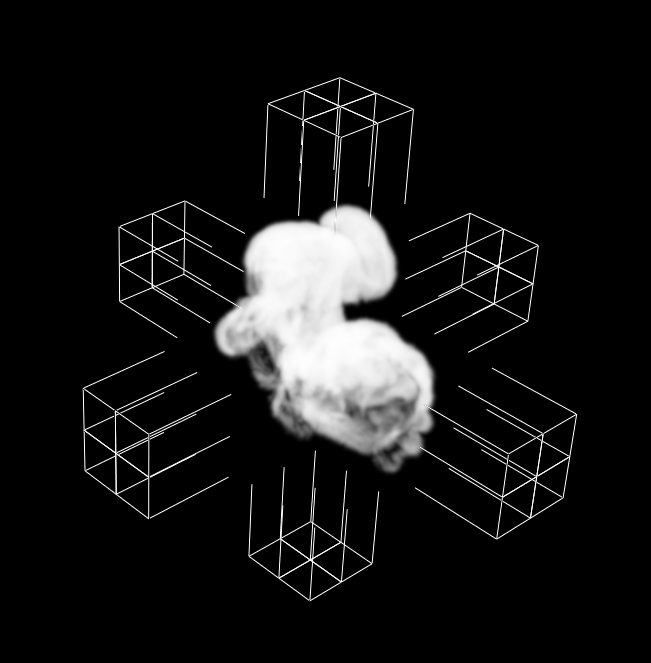
\includegraphics[width=0.49\textwidth]{Grafiken/Implementation/Lightmaps/Smoke_LightSetup.png}
	\centering
	\begin{footnotesize}
		\caption{Setup der 6-Punkt-Beleuchtung einer Rauchsimulation}
		\label{fig:lightSetup}
	\end{footnotesize}
\end{figure}

Die Texturen werden auf zwei verschiedene Arten erstellt. Für die Variante mit Parallax Occlusion Mapping werden drei verschiedene
Texturen, in der von JangaFX entwickelten 3D-VFX-Grafiksoftware EmberGen\footnote{\url{https://jangafx.com/software/embergen/}}, erstellt.
Embergen wurde speziell für Feuer und Rauchsimulationen entwickelt und bietet die Möglichkeit, relativ einfach und schnell, physikalisch basierte und visuell
überzeugende Rauch- und Feuersimulationen zu erstellen (\textbf{\autoref{fig:embergen}}) .
Die Simulationen basieren auf Fluidsimulationen, wodurch ein realistisches Verhalten erzeugt, und durch eine Vielzahl an Parametern beeinflusst werden kann.

Damit der Rauch als Partikel verwendet werden kann, sollte dieser nicht wie eine komplette Rauchfahne, sonder idealerweise wie ein einzelner Rauchball geformt sein.
Bei der Verwendung in einem Partikelsystem können die Partikel dadurch an einem zufälligen Ort mit zufälliger Größe erzeugt und eingeblendet werden. Auf diese
Art wird verhindert, dass der Rauch unnatürlich aussieht. Er bleibt vorallem flexibler was eine mögliche Interaktion des Nutzers mit dem Partikelsystem angeht.
Um einen solchen Rauchball zu erzeugen spielen einige Parameter innerhalb der VFX-Software eine wichtige Rolle. Einer dieser Faktoren ist die Dissipation, also
wie schnell sich der Rauch auflöst. Dieser Wert wurde so hoch wie möglich gestellt, damit der Rauch sich nicht über eine große Fläche zieht, sondern ein kleines Volumen
bleibt. Neben Einstellungen für Force-Fields, um die Simulation etwas zufälliger zu gestalten und Parametern, die sich auf die Dichte, Geschwindigkeit und Druck des Rauchs
und des Feuers beziehen, gibt es eine Vielzahl an Einstellungen für die Domäne in der die Simulation stattfindet. Die Simulation wird auf Basis von Voxeln berechnet.
Es lässt sich festlegen, wie groß das Voxelgitter in X, Y und Z-Richtung sein soll. Dazu lässt sich festlegen, wie groß jedes Voxel für die Berechnung sein soll.
Die Simulation für diese Arbeit wurde in einem 256x256x256 Gitter bei einer Voxelgröße von 10cm durchgeführt. Dies entspricht einer Gesamtanzahl von fast 16.8 Millionen Voxeln.

\begin{figure}[h!]
	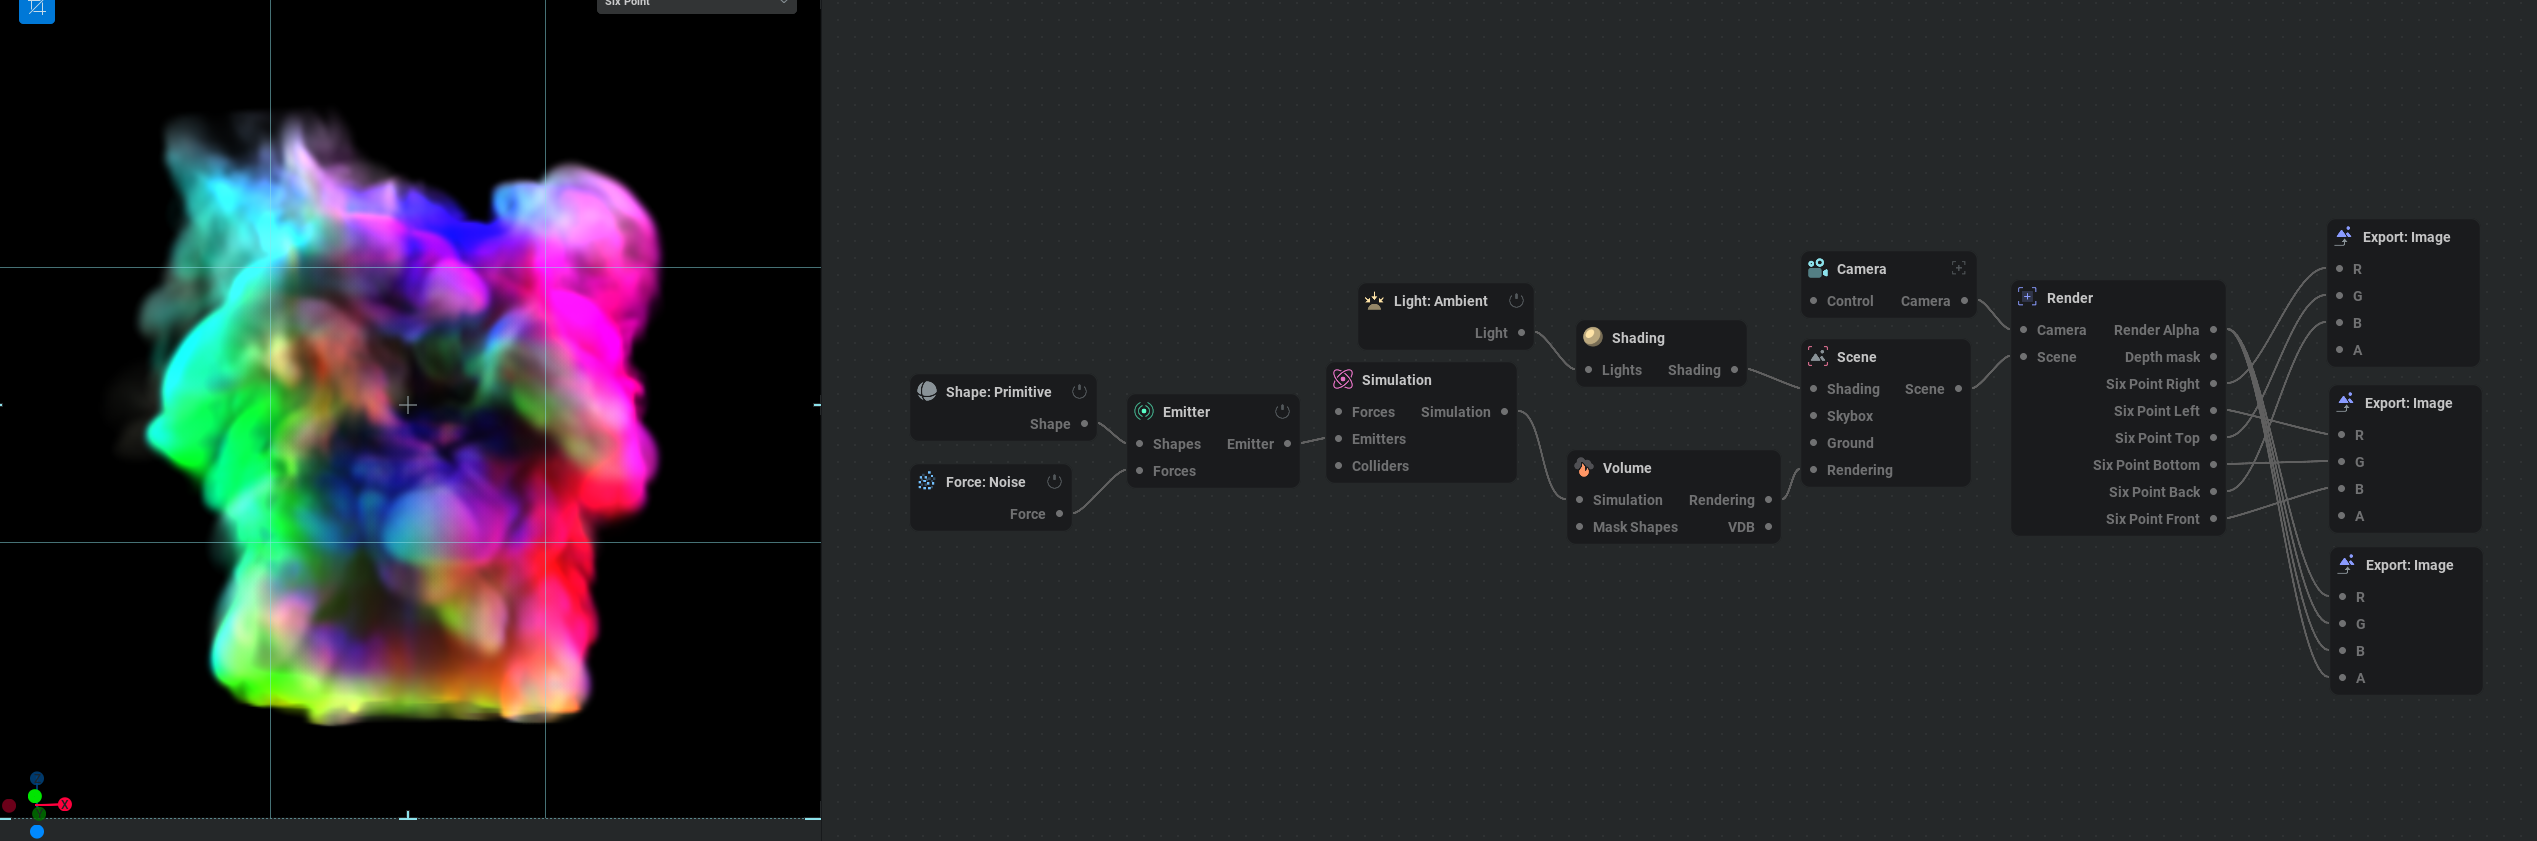
\includegraphics[width=\textwidth]{Grafiken/Implementation/embergen.png}
	\centering
	\begin{footnotesize}
		\caption{Minimales Szenensetup um eine Rauchsimulation zu erzeugen. Auf der linken Seite ist das Ergebnis des Netzwerks auf der rechten Seite zu sehen. Das Shading ergibt sich aus der
			integrierten 6-Punkt-Beleuchtung}
		\label{fig:embergen}
	\end{footnotesize}
\end{figure}

Bei dieser Simulation wird nicht nur die Beleuchtung der Oberfläche aus verschiedenen Richtungen, sondern auch die Streuung, Reflexion und Absorption des Lichts innerhalb
des Volumens berechnet und simuliert.
Eine Möglichkeit die EmberGen bietet, ist das 6-Point Lighting.
Mit dieser Option kann jedes einzelne Licht separat berechnet werden. Dazu werden Lichtquellen wie in \textbf{\autoref{fig:lightSetup}} aus allen sechs Richtungen zum Rauch hin angeordnet,
sodass jeweils eine Seite beleuchtet wird.
Die Animation des Rauches wird daraufhin wie in \textbf{\autoref{fig:seamlessCut}} in eine sich selbst nahtlos wiederholende Animation
geschnitten und als einzelne Frames gerendert. Dazu muss im ersten Schritt eine Animation mit der doppelten Anzahl an Frames erzeugt werden, damit diese in der Hälfte
geschnitten werden kann. Nun werden die beiden Abschnitte übereinander gelegt, sodass sich die Schnittkante auf gegenüberliegenden Seiten befinden. Somit sind der erste
und der letzte Frame nahezu identisch. Als letztes wird ein Crossfade über beide Abschnitte gelegt, wodurch die Clips jeweils an der Schnittkante voll eingeblendet
sind. Das Resultat ist, dass der Schnitt nicht mehr sichtbar und das Video lässt sich unendlich wiederholen. Die Vorteile einer sich endlos wiederholenden Animation werden in \textbf{\autoref{sec:5.1}}
noch weiter erläutert.
Um die verschiedenen Texturlayer in Unity verwenden zu können werden die Lichtrichtungen jedes einzelnen Frames in jeweils einen RGBA-Channel gepackt.
So kann die Ansicht des Rauchs, in der beispielsweise nur die linke Seite beleuchtet wird, in den Roten Kanal einer Textur gespeichert werden.
Dies passiert ebenfalls für die anderen Richtungen von links, unten und oben. Die Ergebnisse sind in \textbf{\autoref{fig:lightDirections}} zu sehen.



\begin{figure}[h!]
	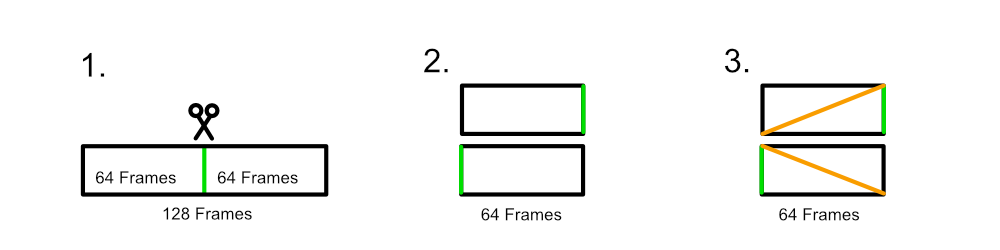
\includegraphics[width=\textwidth]{Grafiken/Implementation/Lightmaps/SeamlessCut.png}
	\centering
	\begin{footnotesize}
		\caption{Schritte um Loop einer Rauchanimation ohne sichtbaren Schnitt zu erzeugen. }
		\label{fig:seamlessCut}
	\end{footnotesize}
\end{figure}

\begin{figure}[h!]
	\centering
	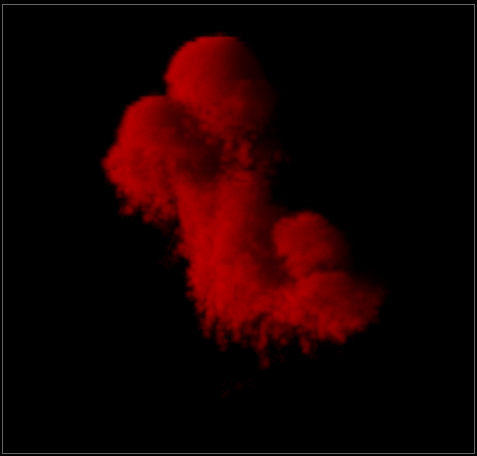
\includegraphics[width=0.19\textwidth]{Grafiken/Implementation/Lightmaps/T1_R.png}
	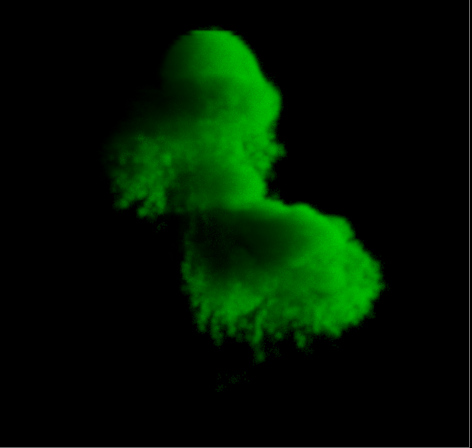
\includegraphics[width=0.19\textwidth]{Grafiken/Implementation/Lightmaps/T1_G.png}
	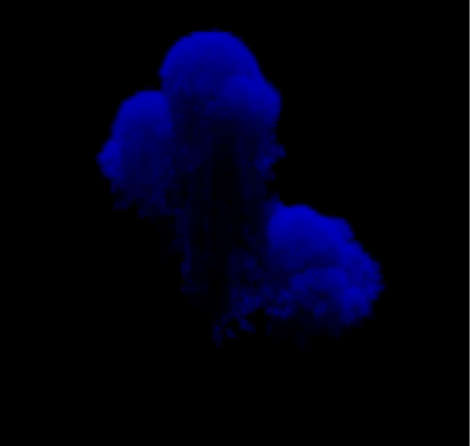
\includegraphics[width=0.19\textwidth]{Grafiken/Implementation/Lightmaps/T1_B.png}
	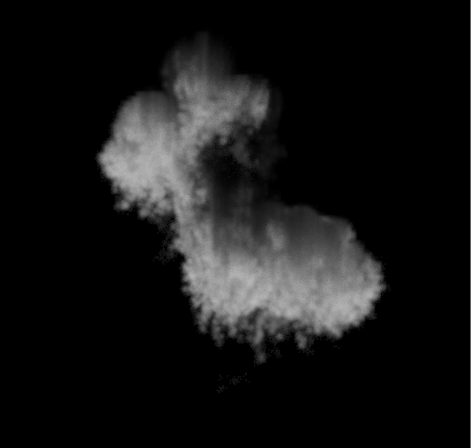
\includegraphics[width=0.19\textwidth]{Grafiken/Implementation/Lightmaps/T1_A.png}
	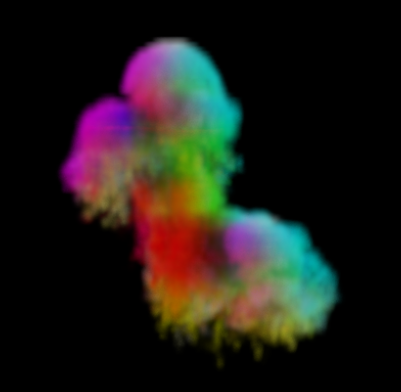
\includegraphics[width=0.19\textwidth]{Grafiken/Implementation/Lightmaps/merged.png}

	\begin{footnotesize}
		\caption{Ein einzelner Frame der Simulation in seine Farbkanäle aufgeteilt. Die Richtungen, aus denen der Rauch jeweils beleuchtet wurde, ist dabei gut zu erkennen.
			Von links: Roter Kanal(links), Grüner Kanal(rechts), Blauer Kanal(oben), Alpha Kanal(unten), Zusammengeführte Textur.}
		\label{fig:lightDirections}
	\end{footnotesize}
\end{figure}


Die verschiedenen Farbkanäle können nun wieder in eine gemeinsame Textur zusammengeführt werden, um dann in Unity in einem Shader weiterverarbeitet zu werden.
Dabei wird jeder Frame mit einer Auflösung von 256x256 Pixeln gespeichert. Bei einer Frameanzahl von 8x8 = 64 Frames entspricht das also
einer Auflösung eines Texture Sheets von 2048 x 2048 Pixeln.

Damit Parallax Occlusion Mapping angewendet werden kann, werden jedoch zusätzlich Informationen über die Höhe oder Tiefe benötigt.
Dazu wird eine weitere Textur mit den gleichen Schritten wie zuvor erzeugt. In diese Textur wird die Tiefenkarte abgespeichert. Zudem kann in ein einem separaten
Farbkanal die Alpha-Information gespeichert werden.


\begin{figure}[hb]
	\centering
	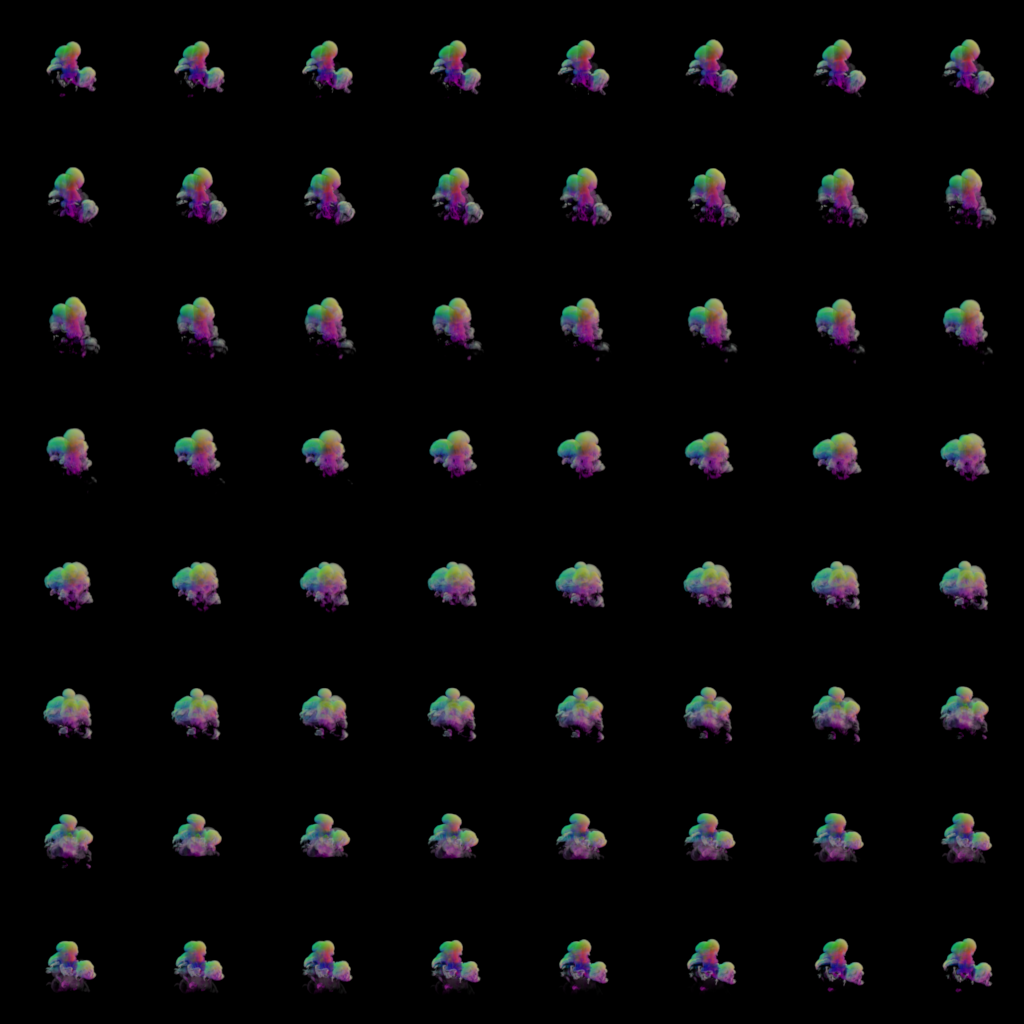
\includegraphics[width=0.49\textwidth]{Grafiken/Implementation/Lightmaps/smokeSim_T1.png}
	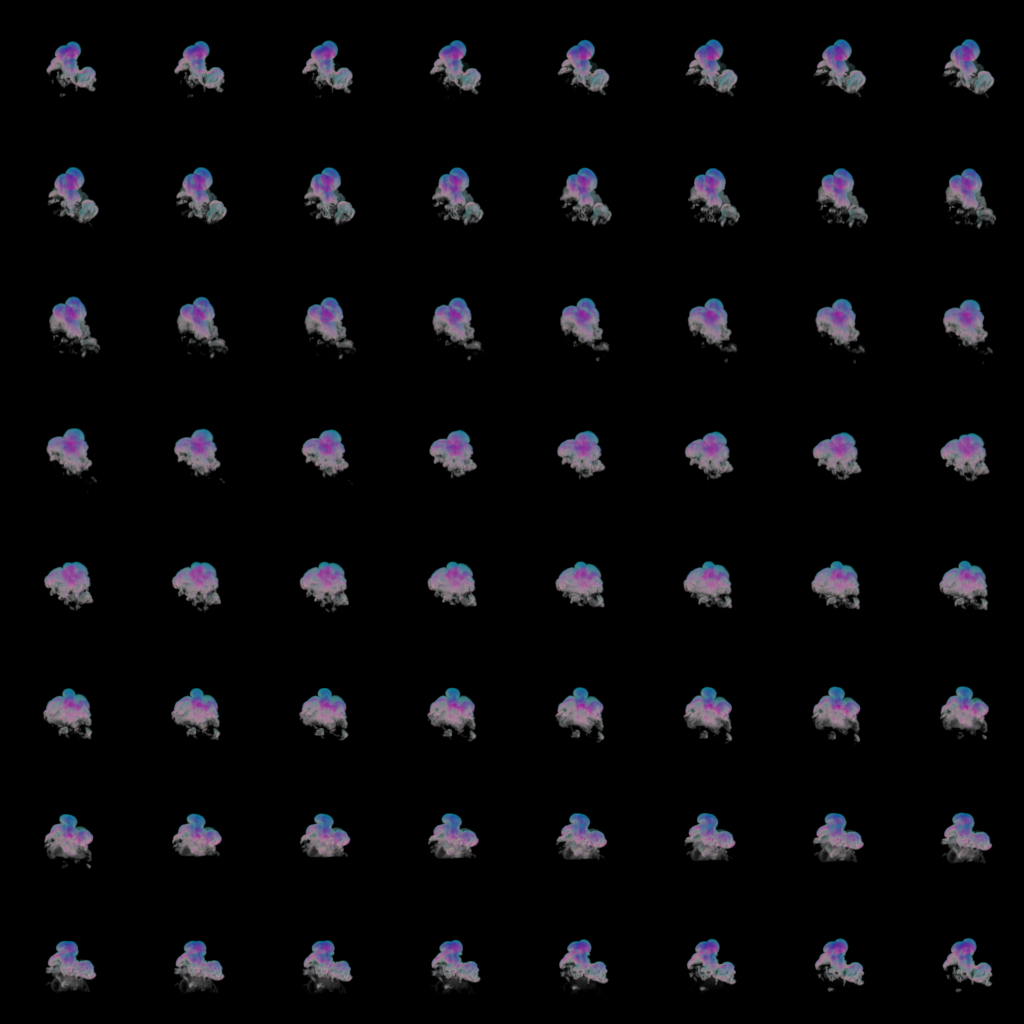
\includegraphics[width=0.49\textwidth]{Grafiken/Implementation/Lightmaps/smokeSim_T2.png}
	\begin{footnotesize}
		\caption{Exportierte Spritesheets aus der Rauchsimulation in Houdini. }
		\label{fig:flipbook}
	\end{footnotesize}
\end{figure}


Für den Ray Marcher wird eine Volumentextur mit Dichtewerten benötigt. Da schrittweise durch das Volumen gelaufen, und dabei überprüft wird, wie viel Licht
durch dieses Volumen wandert, wird hier keine Lichtinformation in der Textur notwendig. Diese wird in Echtzeit von dem Algorithmus berechnet.
Für die Volumentextur kann aus EmberGen, auf Basis derselben Simulation, eine VDB-Datei exportiert werden.
Diese Datei enthält die Volumendaten. Diese kann in der Software Houdini von SideFX importiert werden. Von dort aus lässt sich ein einzelner Frame als Texture Sheet exportieren,
wobei jeder Frame hierbei einen sogennanten Slice des Volumens darstellt. Durch diese Darstellung kann die Information in Unity als 3D-Textur verwendet werden.
Hierbei wird nicht, wie bei der Animation für Parallax Occlusion Mapping, die Zeit als dritte Dimension angesehen, sondern eine weitere räumliche Achse.
Die einzelnen Frames werden übereinander gelegt. Somit bildet diese Textur die Basis für eine statische Rauchwolke, welche durch Ray Marching dargestellt werden kann.





% \subsubsection{Volume Textures}
% TODO


% RAYM: \newline
% - Volumetextures generieren / downloaden\newline
% - Vorgehen beschreiben\newline
% - Grafiken \newline

% % Raymarching: Volumetextures erstellen.
% Diese werden mithilfe von prozedural generierten Noisetexturen erzeugt.
% Daher basiert der zweite Ansatz auf dreidimensionalen Volumentexturen, welche mithilfe von Raymarching gesampled werden.


\subsection{Shader}
Für das Rendering der Partikel werden zwei Shader entwickelt. Diese basieren auf Parallax Occlusion Mapping und auf einem Raymarchingalgorithmus
durch eine Volumentextur. Für POM wird Unitys Shader Graph verwendet. Shader Graph ist, genau wie Unitys VFX Graph, ein Node-Editor um
schnell und übersichtlich Shader zu entwickeln. Dies macht vorallem das Debugging einfacher und erlaubt das schnelle Prototyping von Ideen,
da einiges an Boilerplate-Code erspart wird. Zusätzlich besteht die Möglichkeit auch eigene Funktionen oder HLSL-Files in Nodes
zu verpacken und somit auf visuelle Art und Weise zu entwickeln.


\subsubsection{Parallax Occlusion Mapping}

Um die einzelnen Frames aus den Texture Sheets als Animation darstellen zu können, wird ein
Flipbook-Node\footnote{\url{https://docs.unity3d.com/Packages/com.unity.shadergraph@12.0/manual/Flipbook-Node.html}}
verwendet. Dieser manipuliert die UV-Koordinaten mithilfe der Information über Zeilen und Spalten des Texture Sheets,
sodass die Koordinaten eines jeden Frames abhängig von der Zeit ausgegeben werden.
Somit lässt sich auch die Framerate anpassen, mit der die Animation abgespielt werden soll.

Diese UV-Koordinaten werden nun in einen Parallax Occlusion Mapping-Node weitergegeben, hier wird ebenfalls der Node von
Unity\footnote{\url{https://docs.unity3d.com/Packages/com.unity.shadergraph@12.0/manual/Parallax-Occlusion-Mapping-Node.html}}
benutzt. Dieser berechnet, basierend auf den übergebenen UV-Koordinaten des Flipbook-Players, sowie einer Heightmap und dem Blickwinkel, die anzuzeigenden Texturkoordinaten.
Der Algorithmus mit dem sich das Parallax Offset berechnen lässt wurde in \textbf{\autoref{sec:3.3.4}} erläutert.
Es lassen sich außerdem die Anzahl der Schritte mit denen die Heightmap abgetastet werden soll, sowie die Amplitude des Offsets festlegen.
Für die Implementierung des Rauches wurde die Schrittanzahl auf 150 und die Amplitude auf 1 bis 3.5 gesetzt. Diese Werte haben sich durch Ausprobieren ergeben.
Eine höhere Amplitude lässt Verzerrungsartefakte auftreten.


Da die Beleuchtung des Rauches zuvor in EmberGen durchsimuliert und abgespeichert wurde, muss im Shader nun eine Logik implementiert werden, welche jeweils die richtige Beleuchtung,
abhängig von der Lichtrichtung, anzeigt. Die durch den Flipbook- und POM-Node modifizierten UV-Koordinaten werden nun auf das Texture-Sheet abgebildet und somit die Animation durchlaufen.
Mit der erstellten Animation kann dann unter Einbeziehung des Main Lights (in Unity definiert als die Sonne, also ein directional light) die Richtung, aus der
das Licht kommt, bestimmt werden. Directional Lights haben keine Position, lediglich eine Richtung in die sie zeigen. Mithilfe dieser Richtung kann die korrekte Lightmap
des Rauchs ausgewählt werden oder je nach Richtung des Lichts zwischen verschiedenen Maps interpoliert werden. Im Prinzip wird also für jede Achse des Lichts abgefragt,
in welche Richtung das Licht zeigt. Basierend auf dieser Info kann der entsprechende Farbchannel der Rauchtextur zurückgegeben werden.


\vspace{.6cm}
\begin{lstlisting}[language={[Sharp]C}, label={lst:lightMapLogik}, caption={Logik zur Auswahl der richtigen Lightmap am Beispiel der X-Richtung des Lichts.},captionpos=b, frame=single]
if(lightDirection.X > 0){
  return smokeLightmap_T1.R; 
}
else {
  return smokeLightmap_T2.R; //Licht von links
}

\end{lstlisting}


\subsubsection{Raymarcher}

Da Feuer und Rauch volumetrische Effekte ohne feste Oberfläche sind, lassen sich diese nicht wirklich durch Geometrie abbilden. Die Idee ist also ein
Volumen zu erzeugen und Strahlen durch dieses Volumen zu schicken, welches in festen Abständen das Volumen abtastet, um daraus Informationen zu erhalten.
Hierbei wird das Licht, welches ebenfalls in dieses transluzente Volumen eindringt und absorbiert oder gebrochen wird, an jedem Samplepunkt berechnet.
Die Texturen werden daher wie in \textbf{\autoref{sec:4.1}} beschrieben durch generiertes Rauschen erzeugt.
% Um die notwendige Rechenleistung zu reduzieren, wird auch das generierte Rauschen in Texturen gebacken.  

Der Algorithmus des Ray Marchers schickt Strahlen von der Kamera durch jeden Pixel. Wird ein Objekt getroffen, so wird mit einer festgelegten Schrittweite
inkrementell das Volumen durchlaufen. Dabei werden an jedem Punkt die Werte für die Dichte aus den Textur Slices, die das Volumen darstellen, gelesen. Zudem
wird das Licht, welches den jeweiligen Punkt im Volumen erreicht mit gespeichert. Dies gelingt durch einen Ray Cast von dem abgetasteten Punkt in Richtung der Lichtquelle.

Für den Shader wird ein Custom Function-Node für das Marching erzeugt. Der Algorithmus läuft die in \textbf{\autoref{alg:rayM}} grob zusammengefassten Schritte für jeden Strahl durch:


\begin{algorithm}
	\caption{Volume Ray Marching Algorithmus.}\label{alg:rayM}
	\begin{algorithmic}

		\For {every sample point $P_i$ along viewing ray $\vec{v}$}
		\State $density$ += sampledTextureDensity
		\State Cast ray $\vec{l}$ from sample point to light position
		\For {every sample point $L_j$ on $\vec{l}$}
		\State $lighting$ += sampledLightDensity
		\EndFor
		\EndFor
		\State color = (density, lighting, 0)
	\end{algorithmic}
\end{algorithm}

Ray Marching Algorithmus:  → Nur Notizen für mich :)  \\
- Ray Cast in Volumen.\\
- An jedem Sample: \\ \textit{
	- Dichte auslesen\\
	- Ray Cast zur Lichtquelle\\
	- Daraus berechnen wie viel Licht ankommt\\
	- mit der Dichte verrechnen\\
	- Nächster Schritt\\
}
- Alle Werte auf einem Strahl zusammen rechnen\\

\subsection{Partikelsystem}
Um die Partikelsysteme umzusetzen, wird der relativ junge, von Unity entwickelte Editor 'Visual Effects Graph'
(kurz: VFX Graph), verwendet. VFX Graph ist ein nodesbasierter Editor, um schnell
dynamische und komplexe Partikelsysteme zu erzeugen\footnote{\url{https://unity.com/de/visual-effect-graph}}.
Im Gegensatz zum älteren Shuriken-Partikelsystem von Unity werden die Partikel hier auf der GPU
simuliert, wodurch das System deutlich an Performance gewinnt und daher mehr Partikel zeichnen kann.
Shuriken nimmt die Berechnungen im Gegensatz zum VFX Graph auf der CPU vor\footnote{\url{https://docs.unity3d.com/Manual/ChoosingYourParticleSystem.html}}.
Gerade für VR-Anwendungen bietet sich also dieses neue System an.
VFX-Graph hat jedoch nur sehr begrenzte Möglichkeiten, was Physiksimulationen und Kollisionen der Partikel angeht.
Es muss also ein System erstellt werden, welches trotz der Einschränkungen ein möglichst realistisches
Verhalten der Feuer- und Rauchpartikel gewährleistet.




\newpage
